\chapter{Sviluppo Piattaforma}
\label{chp:sviluppo}

L'analisi dei requisiti ha evidenziato la necessità di un sito web in cui esporre e descrivere al cliente i servizi offerti, aggiornato e popolato da un componente del team di {\fem} senza per forza conoscenze e capacità tecniche informatiche; si é scelto quindi WordPress, un CMS molto diffuso.

Per la gestione degli ordini sia dal lato cliente che dal lato admin invece é stata progettata un soluzione su misura, utilizzando \emph{Django}, un web framework per lo sviluppo di applicazioni web. 

La mole di lavoro da compiere ha creato la necessita di dividere i compiti, così io mi sono occupato dello sviluppo lato client/front-end dell'applicativo e del controllo del CMS {\wp}; il lato server é stato invece compito di due colleghi.

In questo capitolo verranno descritti ed analizzati tutti i passi fino alla messa online del sito con particolare attenzione al lato front-end. Nel dettaglio la sezione \ref{sec:wp} descriverà le azioni per impostare correttamente il CMS, la sezione \ref{sec:server} fornirà una panoramica sul lato server, mentre il lato client sarà descritto più dettagliatamente nella sezione \ref{sec:client}.

% --WordPress--
\section{WordPress}
\label{sec:wp}

{\wp} è una piattaforma software di content management system (CMS) ovvero un programma installato sul server che consente la creazione, gestione, distribuzione e manutenzione di un sito Internet \cite{wordpress}. É un progetto open-source creato da Matt Mullenweg e distribuito con la licenza GNU General Public License; é sviluppato in PHP con appoggio a MySQL come gestore di database.

{\wp} permette il download gratuito di tutti i suoi componenti dal sito \url{www.wordpress.org} per poterli installare sulla propria macchina. Esiste anche un servizio (a pagamento in base alle richieste) chiamato \emph{WordPress.com} che permette di costruire rapidamente il proprio sito web o blog basato su {\wp} senza la necessità di possedere un server o competenze tecniche specifiche.

\subsection{Caratteristiche di {\wp}}

{\wp} permette di estendere le proprie funzionalità con l'ausilio di opportuni plugin, ovvero moduli che aggiungono nuove caratteristiche ed elementi all'applicativo. I plugin possono essere gratuiti o a pagamento e possono fare molte fare di tutto, dal potenziare l'editor integrato di {\wp} all'inserire slideshow nelle pagine, e molto altro ancora. Come i plugin si possono trovare anche temi, estensioni che permettono di personalizzare l'aspetto del sito modificando sfondi, impaginazione, font, etc.

\subsection{{\wp} per {\fem}}

Per realizzare il \emph{Portale della Diagnostica Molecolare dedicato all'Avifauna}, dopo aver scelto il sottodominio \texttt{www.avifauna.fem2ambiente.com}, si é prima di tutto installato e configurato {\wp}.

Per farlo é stato necessario scaricare l'ultima versione dal sito \url{www.wordpress.org} (ad oggi, Ottobre 2015, l'ultima versione é la 4.3.1) e seguire le istruzioni nel file \texttt{readme} \cite{installing_wordpress}, in particolare:
\begin{itemize}
\item eseguire le opportune modifiche al file \texttt{wp-config.php} in un editor di testo;
\item creare un database dedicato utilizzando MySQL;
\item connettersi al server e caricare tutti i file relativi l'installazione di {\wp} nella cartella scelta (\texttt{/home});
\item configurare in modo appropriato visitando la pagina 

\texttt{http://avifauna.fem2mabiente.com/home/wp-admin/install.php}
\end{itemize}

Una volta terminata l'installazione si é potuto procedere con l'installazione degli appropriati plugin, temi e estensioni.

La scelta del tema é ricaduta su \emph{Everest} di YOOtheme (Versione: 1.0.11). YOOtheme é una azienda tedesca che produce componenti per CMS \cite{yootheme}; i loro prodotti più importanti, oltre a una ventina di temi e template diversi rispettivamente per {\wp} e Joomla!, sono \emph{Wrap Framework} \cite{wrap} e \emph{Uikit} \cite{uikit}, due architetture software di supporto per la creazione e personalizzazione dei componenti aggiuntivi ai più famosi CMS.

Il tema Everest é stato costruito utilizzando Wrap Framework e mette a disposizione dell'utilizzatore sette stili di layout differenti, personalizzazioni nella costruzione del layout sfruttando tutte le potenzialità di {\wp} e un pacchetto di plugin chiamato \emph{Widgetkit} per l'inserimento rapido di Slideshow, gallierie di immagini, mappe. Per tutte queste caratteristiche é stato scelto, acquistato ed installato come tema per il sito.

Per ricoprire tutti i bisogni organizzativi di un sito commerciale come il Portale Avifauna é stato necessario installare anche plugin come \emph{Polylang} \cite{polylang} per il supporto multilingue al sito e \emph{My Calendar} \cite{mycalendar} per la gestione degli eventi.

Dopo aver creato popolato il sito con i contenuti, divisi in base alle pagine e sezioni dedicate, il risultato ottenuto é visibile nell'immagine~\ref{fig:homepage} e al seguente link \url{www.avifauna.fem2mabiente.com/home}.

\begin{figure}
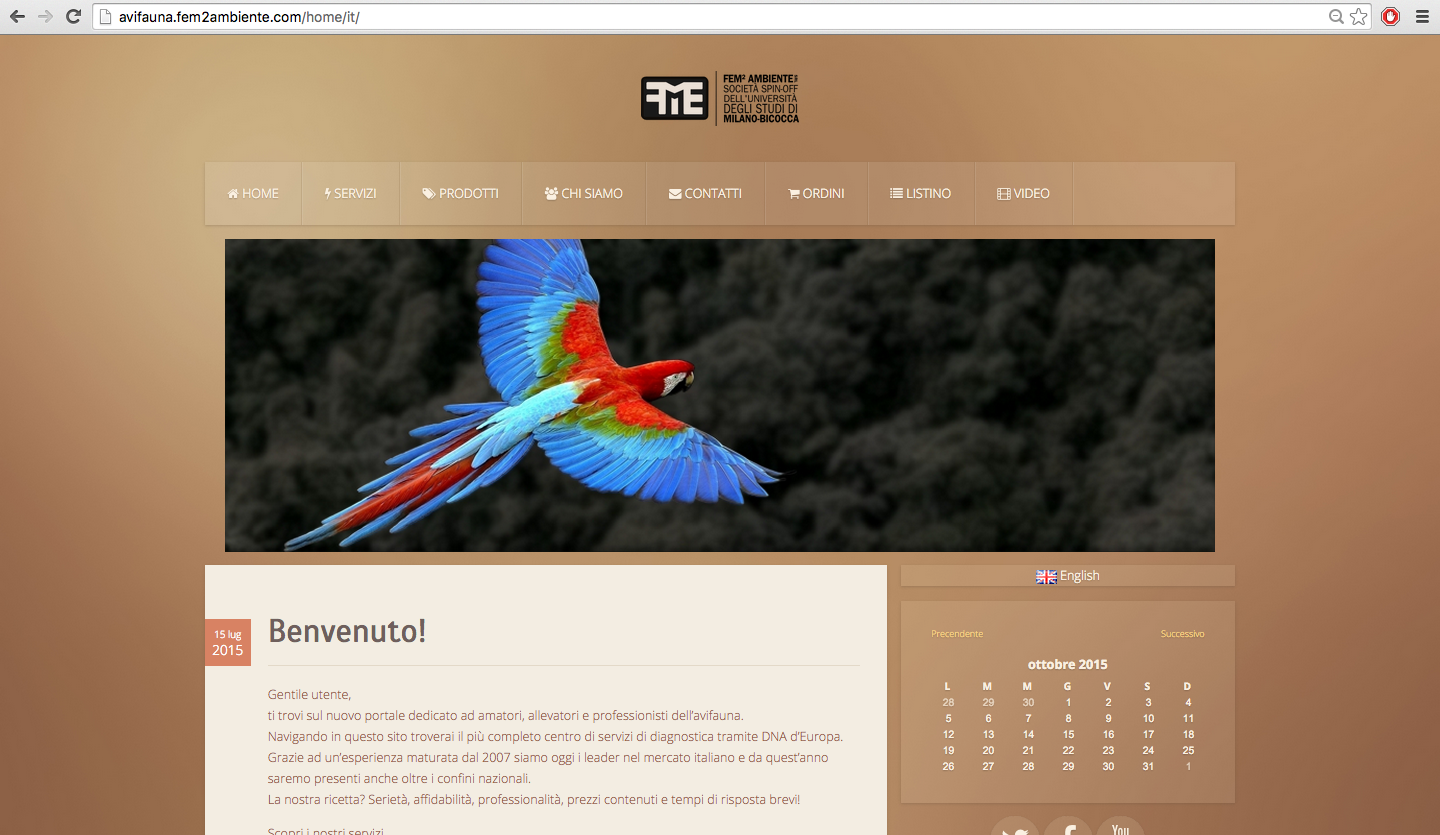
\includegraphics[width=1\textwidth]{images/homepage} 
\caption{homepage del Portale per la Diagnostica Molecolare Avifauna}
\label{fig:homepage}
\end{figure}

Cliccando sul tasto \textsf{Ordini} si può accedere alla piattaforma personalizzata, descritta nei seguenti capitoli.

\begin{center}

\includegraphics[width=0.3\textwidth]{images/homepage-ordini} 
\label{fig:homepage-ordini}
\end{center}

% --Lato Server--
\section{Lato Server}
\label{sec:server}
Per lo sviluppo della piattaforma web le tecnologie utilizzate sono state: \emph{Django} come web framework e MySQL e SQLite per il database.

\subsection{Django}
\label{django}
\emph{Django} è un web framework open source per lo sviluppo di applicazioni web, scritto in linguaggio \emph{Python}; il progetto è sviluppato dalla "Django Software Foundation" (DSF), un'organizzazione indipendente senza scopo di lucro \cite{django}. É stato inizialemente concepito per gestire diversi siti di notizie, ed in seguito distributo con una licenza BSD (Berkeley Software Distribution) a luglio 2005.

La scelta di Django é ricaduta grazie alle molte proprietà: dall'astrazione del database relazionale ad oggetti, alla
possibilità di installare funzionalità attraverso plugin, dalla robusta API per la gestione del database, al sistema di "view generiche" che evitano la stesura di codice ripetitivo per determinati casi comuni e soprattutto il sistema di template  e gestore di URL basate su espressioni regolari. Django offre inoltre un efficace supporto per localizzazione, incluse traduzioni dell'interfaccia amministrativa in molte lingue.

\subsection{Configurazione}
Il primo passo é stato l'installazione delle componenti di Django, attraverso la creazione del progetto (nome di esempio \texttt{mysite}), con il comando a terminale:
\begin{verbatim}
$ django-admin startproject mysite
\end{verbatim}

così da ottenere la seguente configurazione di file:
\begin{small}
\begin{verbatim}
mysite/
    manage.py
    mysite/
        __init__.py
        settings.py
        urls.py
        wsgi.py
\end{verbatim}
\end{small}

Abbiamo quindi impostato nel file \texttt{settings.py} il database scelto, le lingue del sistema, il percorso dei file statici, dei media e le \texttt{INSTALLED\_APPS}.

Le \texttt{INSTALLED\_APPS} sono una sorta di librerie usate per l'aggiunta di componenti al progetto costruito; le più importanti sono:
\begin{itemize}
 \item \texttt{django.contrib.admin} - il creatore automatico del pannello admin
 \item \texttt{django.contrib.auth} - il sistema di autenticazione
 \item \texttt{django.contrib.sessions} - il framework per il controllo delle sessioni
 \item \texttt{django.contrib.messages} - il framework di controllo per i messaggi
 \item \texttt{django.contrib.staticfiles} - il gestore dei "file statici"
\end{itemize}

\subsection{Creazione}
Durante tutta la fase di sviluppo é stato necessario avviare il \emph{development server} attraverso il comando da terminale:
\begin{verbatim}
$ python manage.py runserver
\end{verbatim}
per simulare il comportamento del server in modo da generare il sito all'indirizzo \texttt{http://127.0.0.1:8000/} .

Una componente fondamentale é rappresentata dai \emph{modelli}, strutture associabili concettualmente alle classi in Java; in funzione alle richieste avanzate da {\fem} il diagramma in figura (BOH) rappresenta come sono stati configurati i modelli con i relativi attributi.

SCHEMA STRUTTURA MODELLI

Di seguito sono descritti i principali modelli.

\subsection*{clienti.py}
\label{subs:clienti}
Il cliente é un componente delicato ed importante del sistema. 

L'attributo \texttt{tipo} é necessario in quanto per {\fem} il cliente può essere differenziato in quattro tipi: Amatore, Allevatore, Veterinario e Negozio. Esso é identificato univocamente dall'indirizzo \texttt{email} inserito al momento della registrazione e ha chiaramente un attributo \texttt{ragione\_sociale} per indicare nome e cognome per un privato, oppure ragione sociale in caso contrario. Ogni cliente ha altri numerosi attributi per ogni dato personale relativo all'indirizzo (necessario per la spedizione degli attestati generati al termine delle analisi), contatti telefonici e \texttt{lingua\_preferita} per tradurre il sistema correttamente.

Ogni cliente può acquistare pacchetti di \emph{Crediti FEM}, cioè una somma di denaro pronta per gli acquisti pagata anticipatamente, in modo da non dover effettuare il pagamento al termine di ogni ordine, é quindi necessario indicare la quantità di crediti posseduta da ogni cliente in un apposito attributo.

Infine ogni cliente può essere iscritto ad una associazione convenzionata all'azienda {\fem} e deve poter inserire il proprio numero di tessera per accedere agli sconti relativi; per farlo si deve dare uno sguardo ai modelli \texttt{associazioni.py} e \texttt{prezzi.py}.

\subsection*{prezzi.py}
\label{subs:prezzi}
Ogni \texttt{SchemaPrezzi} é identificato dal \texttt{nome} e può essere associato a nessuno, uno o tanti clienti. Esso definisce i costi fissi delle commissioni per ogni metodo di pagamento scelto, il prezzo degli attestati e il prezzo di ogni analisi, che tendenzialmente può variare tra uno SchemaPrezzi e l'altro.
In particolare abbiamo deciso di differenziare gli SchemaPrezzi secondo una caratteristica principale: se schema \emph{Pacchetti} o \emph{Convenzioni}.

Uno SchemaPrezzi del tipo \emph{Pacchetti} é caratteristico di un cliente standard, che può usufruire di sconti vincolati a quantità, ad esempio con l'acquisto di un analisi APV associato ad un analisi SMAP riduce il costo di entrambe. Uno SchemaPrezzi del tipo \emph{Convenzioni} invece é adatto per i clienti che risultano iscritti ad una associazione che ha attiva una convenzione con {\fem}; questo tipo di SchemaPrezzi modifica il prezzo di tutte o alcune analisi anche in relazione alle specie del campione scelta.

\subsection*{associazioni.py}
\label{subs:associazioni}
Una \texttt{Associazione} é caratterizzata da un nome e da uno schema prezzi associato. \texttt{IscrizioneAssociazione} indica la correlazione tra un cliente, indicato attraverso nome e numero di tessera, e una associazione.

\subsection*{ordini.py}
\label{subs:ordini}
L' \texttt{Ordine} é il componente più delicato e complesso del sistema a causa del suo flusso rappresentato in figura (BOH).

Esso é caratterizzato da un numero, dal \texttt{cliente} che l'ha creato e dall''attributo \texttt{stato} che indica in quale posizione del flusso si trova.
Altri attributi interessanti sono:
\begin{itemize}
 \item \texttt{metodo\_pagamento} indica il metodo di pagamento scelto
 \item \texttt{totale\_servizi} indica il costo delle analisi richieste con aggiunte le eventuali spese di spedizione per gli attestati cartacei 
 \item \texttt{crediti\_consumati} indica la quantità di crediti FEM utilizzati per pagare l'ordine
 \item \texttt{servizi\_da\_pagare} indica il  \texttt{totale\_servizi} da cui sono stati sottratti i \texttt{crediti\_consumati}
 \item \texttt{ammontare} indica il \texttt{totale\_servizi} sommato all'eventuale costo di commissione previsto dal metodo di pagamento
\end{itemize}

\subsection*{specie.py}
\label{subs:specie}

\begin{wrapfigure}{r}{0.3\textwidth}
 \begin{center} 	
  \begin{scriptsize}
   \begin{itemize}
    \item Dominio
    \item Regno
     \begin{itemize}[label=$\bullet$]
      \item Sottoregno
     \end{itemize}
    \item Phylum
     \begin{itemize}[label=$\bullet$]
      \item Subphylum
     \end{itemize}
    \item Classe
     \begin{itemize}[label=$\bullet$]
      \item Sottoclasse
     \end{itemize}
    \item Ordine 
     \begin{itemize}[label=$\bullet$]
      \item Sottordine
     \end{itemize}
    \item Famiglia
     \begin{itemize}[label=$\bullet$]
      \item Sottofamiglia
     \end{itemize}
    \item Genere
     \begin{itemize}[label=$\bullet$]
      \item Sottogenere
     \end{itemize}
    \item Specie
	 \begin{itemize}[label=$\bullet$]
	  \item Sottospecie
	 \end{itemize}
    \item Clade e Coorte
   \end{itemize}
  \end{scriptsize}    	
 \end{center}
\caption{Classificazione tassonomica}
\label{fig:tassonomia}
\end{wrapfigure}

É necessario prima di tutto spiegare che la tassonomia (dal greco \emph{taxis} "ordinamento", e \emph{nomos} "norma" o "regola") é definita in generale come la disciplina della classificazione. Abitualmente si impiega il termine per indicare la tassonomia biologica, ossia la disciplina scientifica che si occupa di attribuire un nome agli organismi viventi e di classificarli.  La classificazione tassonomica può essere descritta come in figura~\ref{fig:tassonomia}.

Per classificare tutti i po







% --Lato Client--
\section{Lato Client}
\label{sec:client}
uooo